\documentclass[11pt]{amsart}
%prepared in AMSLaTeX, under LaTeX2e
\addtolength{\oddsidemargin}{-.85in}
\addtolength{\evensidemargin}{-.85in}
\addtolength{\topmargin}{-.5in}
\addtolength{\textwidth}{1.7in}
\addtolength{\textheight}{1.1in}
\newcommand{\normalspacing}{\renewcommand{\baselinestretch}{1.05}
        \tiny\normalsize}

\newtheorem*{thm}{Theorem}
\newtheorem*{lem}{Lemma}
\newtheorem*{defn}{Definition}
\newtheorem*{example}{Example}
\newtheorem*{problem}{Problem}
\newtheorem*{remark}{Remark}

\usepackage{amssymb,verbatim,alltt,xspace}
\newcommand{\mtt}{\texttt}

\usepackage{fancyvrb}
\newcommand{\mfile}[1]{
\begin{quote}
\bigskip \bigskip
%\VerbatimInput[frame=single]{#1}
\VerbatimInput[frame=single,label=\fbox{\normalsize \textsl{\,#1\,}},fontfamily=courier,fontsize=\small]{#1}
\end{quote}
\bigskip
}

\usepackage[final]{graphicx}
%{\includegraphics[width=3.2in,keepaspectratio=true]{#1}}


% macros
\newcommand{\CC}{\mathbb{C}}
\newcommand{\Div}{\nabla\cdot}
\newcommand{\eps}{\epsilon}
\newcommand{\grad}{\nabla}
\newcommand{\ZZ}{\mathbb{Z}}
\newcommand{\ip}[2]{\ensuremath{\left<#1,#2\right>}}
\newcommand{\lam}{\lambda}
\newcommand{\lap}{\triangle}
\newcommand{\RR}{\mathbb{R}}

\newcommand{\bb}{\mathbf{b}}
\newcommand{\bx}{\mathbf{x}}
\newcommand{\by}{\mathbf{y}}
\newcommand{\bz}{\mathbf{z}}

\newcommand{\tb}{\textsc{Morton \& Mayers 2nd ed}}
\newcommand{\pexer}[2]{\bigskip\noindent\textbf{#1.} (Exercise #2 in \tb.)}
\newcommand{\prob}[1]{\bigskip\noindent\textbf{#1.} }
\newcommand{\epart}[1]{\medskip\noindent\textbf{(#1)} }
\newcommand{\note}[1]{[\scriptsize #1 \normalsize]}

\newcommand{\Matlab}{\textsc{Matlab}\xspace}
\newcommand{\Octave}{\textsc{Octave}\xspace}
\newcommand{\pylab}{\textsc{pylab}\xspace}
\newcommand{\MOP}{\textsc{MOP}\xspace}


\begin{document}
\scriptsize \noindent Math 615 Numerical Analysis of DEs \hfill Bueler; \today
\bigskip

\Large\centerline{\textbf{Solutions to Assignment \#5}}
\medskip
\small
\begin{quote}
\emph{These problems are from the} Two-point Boundary Value Problems: Numerical Approaches \emph{slides.  The first two problems were worth 5 points each.  The second two problems were worth 10 points each.  The total is 30 points}.
\end{quote}
\normalsize
\medskip
\thispagestyle{empty}
\normalspacing

\prob{Exercise 1}  (\emph{Easy warm-up.})  The characteristic polynomial is $m^2+2m+2=0$ with roots $m=(-2\pm\sqrt{-4})/2 = -1 \pm i$ so the general solution is $y = c_1 e^{-x} \cos x + c_2 e^{-x} \sin x$.  The boundary conditions are these equations:
\begin{align*}
  1\, c_1+ 0\, c_2 &= 1, \\
  e^{-1}\cos 1\, c_1 + e^{-1} \sin 1\, c_2 &= 0.
\end{align*}
These linear equations have a unique solution.  The solution is $c_1 = 1$ and $c_2 = - (\cos 1)/(\sin 1) = - \cot 1 = - 0.64209$, so
	$$y(x) = e^{-x}\left(\cos x - 0.64209 \sin x\right).$$

\prob{Exercise 2}  (\emph{Also easy, but it makes this point:  When the linear two-point BVP has certain boundary values for which there are \emph{no} solutions, then once once considers the boundary values for which there \emph{are} solutions, one finds infinitely-many solutions.  This is the \emph{Fredholm alternative}.})

The general solution of the ODE is $y(x) = c_1 \cos \pi x + c_2 \sin \pi x$.  The boundary conditions say $c_1=1$ and $c_1 \cos \pi + c_2 \sin \pi = A$ or $- 1 = A$.  Thus there are solutions when $A=-1$, in which case $c_2$ is free to be anything it wants; these are infinitely-many solutions to the twopoint BVP:
	$$y(x) = \cos\pi x + c_2 \sin \pi x,$$
where any value of $c_2$ is allowed.

Something like this same situation happens in linear algebra.  In particular, if $M$ is a matrix, and if we seek vector solutions $\bx$ to $M \bx = \lambda \bx$, then we find that there are no nonzero solutions $\bx$ for most values of $\lambda$.  But if we choose the right value of $\lambda$, an eigenvalue, then $M\bx = \lambda \bx$ allows infinitely many solutions $\bx$, the eigenvectors.  The two-point BVP above, which has nonhomogeneous boundary values,  corresponds to solving $M\bz - \lambda \bz = \bb$ for some nonzero right-hand side $\bb$.  (Here $\lambda = -\pi^2$ and $M$ corresponds to the operation ``$d^2/dx^2$''.)  Once $\lambda$ is chosen to be an eigenvalue of $M$ then there is a restriction on $\bb$ so that nonzero solutions $\bz$ exist, but if that restriction is satisfied then one can add an arbitrary eigenvector $\bx$ of $M$ with eigenvalue $\lambda$ to any solution.  That is, if $\bz$ is a solution then so is $\by = \bz + c \bx$.

\prob{Exercise 3}  To solve this ODE BVP by finite differences, I started from the code shown on slide 26.  The key modifications are indicated by this one line giving the finite difference version of the ODE:
	$$Y_{j-1} + \left(-2 + \Delta x^2\,\sin(5x_j)\right) Y_j + Y_{j+1} = \Delta x^2\,\left(x_j^3 - x_j\right), \qquad j=1,\dots,J-1,$$
along with $Y_0=0$ and $Y_J=0$.  The code looks like this, noting that indices go from $1$ to $J+1$:

\mfile{exer3.m}

The output looks like this:
\medskip

\begin{center}
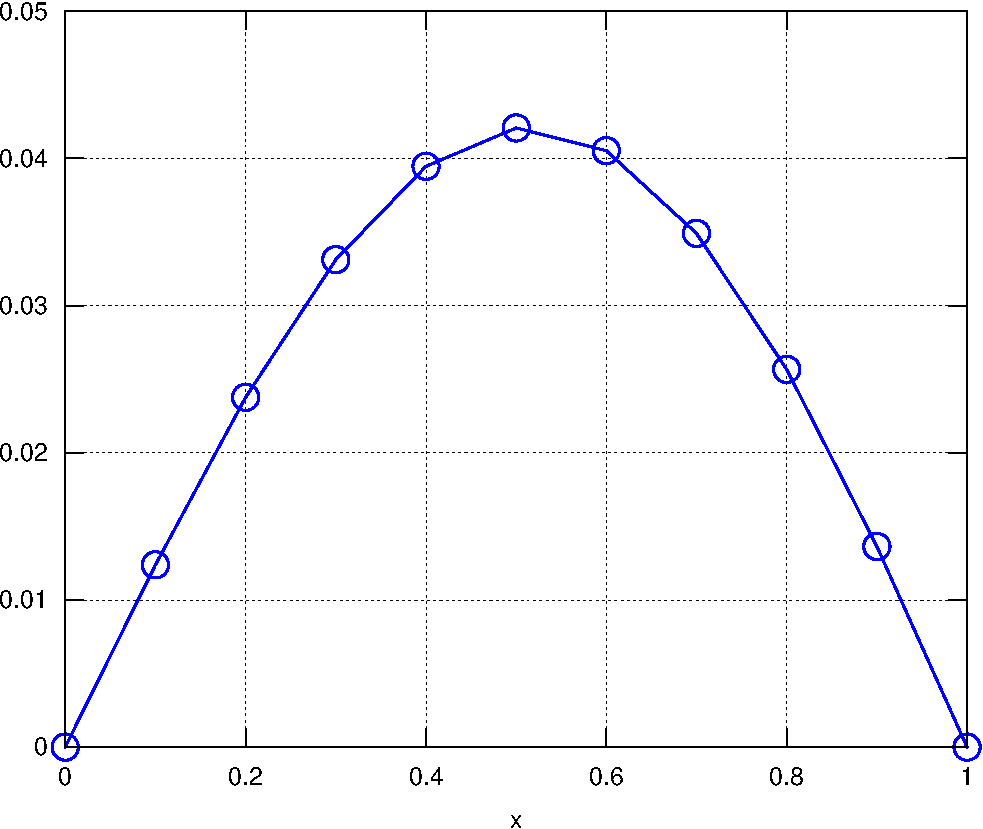
\includegraphics[width=3.0in,keepaspectratio=true]{exer3}
\end{center}
\medskip

\large\emph{Are we right?}\normalsize\,  We are in a fairly-generic situation.  We have written a code to approximately solve a problem which is sufficiently-difficult that we do not know the exact solution.  How do we tell that the code is right?

Here is a fundamental, generic, and often-forgotten suggestion: 
\begin{quote}
\emph{We can usually modify the code just slightly to solve both the problem we are interested in, and a nearby problem to which we know the exact solution.}
\end{quote}
Concretely, note that the picture looks somewhat like the function $v(x) = \sin(\pi x)$.  Let's substitute that into the left side of the ODE to see what right-hand side would make an equality.  This is known as \emph{manufacturing} a nearby ODE problem to which we know the exact solution:
	$$v'' + \sin(5 x) v \stackrel{\ast}{=} \sin(\pi x) \left(\sin(5 x) - \pi^2\right).$$
That is, $v(x) = \sin(\pi x)$ now solves ODE $\ast$, an ODE which differs from the ODE we \emph{want} to solve merely by having a different right-hand side.  Note $v(x)$ also has the same boundary values as our desired solution, $v(0)=0$ and $v(1)=0$.

So here is a code that is trivially different from \texttt{exer3.m}.  As shown in the examples in its comments, it can both solve the \textbf{Exercise 3} problem and the problem $\ast$, on which we can measure the error:

\mfile{exer3safe.m}

Running this on finer and finer grids (i.e.~$J=10,10^2,10^3,10^4$) gives great evidence of success.  To make this efficient I wrote yet another code, that calls \texttt{exer3safe.m}:

\mfile{exer3analysis.m}

Running it gives
\small
\begin{quote}
\begin{verbatim}
>> exer3analysis
ans =
                    10     0.008638049173471
                   100  8.59448228660575e-05
                  1000  8.59407540687585e-07
                 10000  8.58439119788557e-09
\end{verbatim}
\end{quote}
\normalsize
Thus we see that the error decreases by about 6 orders of magnitude as we increase $J$ from $10$ to $10^4$, i.e.~by 3 orders of magnitude.  This is the signature of a correctly-implemented $O(\Delta x^2)$ method.

\prob{Exercise 4}  I wrote the following code:

\mfile{nonlinshow.m}

\noindent The figure that results is this:

\bigskip
\begin{center}
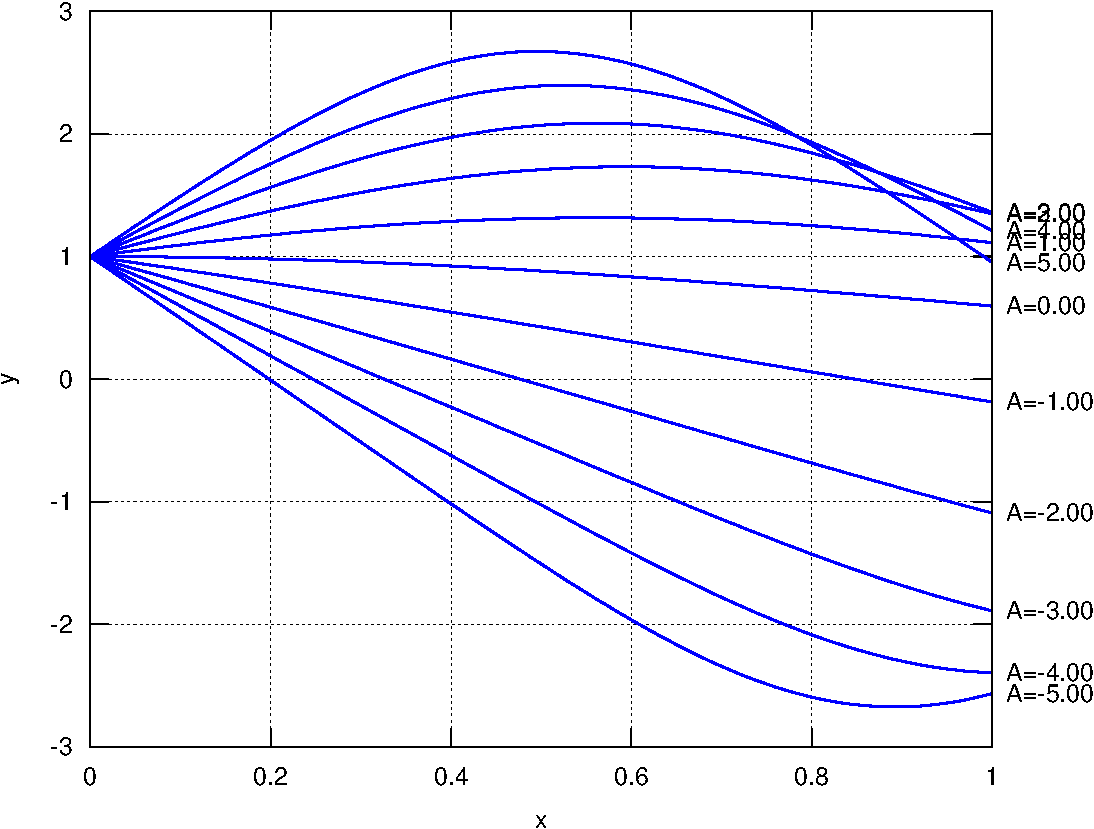
\includegraphics[width=4.5in,keepaspectratio=true]{nonlinshow}
\end{center}

\noindent I conclude that the solution of the BVP with $u(1)=-2$ would come from solving the ODE IVP with $u'(0)=A$ between $A=-3.0$ and $A=-4.0$.  From the picture, $A=-3.2$ might be a good guess.

Our bracket $-3.0 \le A \le 4.0$ is exactly the info needed to run the bisection algorithm.  See

\centerline{\texttt{nonlinbisect.m}}

\noindent posted online for such a bisection-using code for this problem.  It gets $A=-3.172654927072$.

\end{document}

